\chapter{Konzept}

\section{Detaillierter Gesten-Steuerbeschrieb}
\label{sec:gestureControll}

Ziel dieser Steuerung ist es, die Drohne sehr einfach steuern zu können.
Das auswendig Lernen der möglichen Gesten soll durch intuitive Schlussfolgerungen des Anwendungswunsches entfallen.
Der Grundgedanke der Steuerung soll die Hand sein, welche die Drohne verkörpert.

\begin{framed}
\textit{Definition: }\textbf{Position}\\
Im Folgenden ist mit dem Begriff \textit{Position} jeweils die dreidimensionale Ausrichtung im Raum und nicht der effektive Standort gemeint.
\end{framed}

\subsection{Leap Motion}
%todo correct
Es folgt eine grobe Übersicht des Gestenerkennungs-Sensores \textit{Leap Motion}.
Detailliertere Informationen sind im \secref{subsec:leapmotion} zu finden.
% Es folgen grobe Informationen zum Gestenerkennungs-Sensor \textit{Leap Motion}.

Der Sensor erkennt Gesten innerhalb eines 150\textdegree-Winkels zwischen 25\,mm und 600\,mm Höhe.
Um genügend vertikale Spatzung für den Höhenunterschied zu bewahren, soll die Steuerung auf 10 --  35\,cm Höhe initialisiert werden.
Folgend wird auf die grundlegenden Flugmanöver eingegangen.

\subsection{Flugmanöver}
\begin{framed}
	\textit{Bemerkung: }\textbf{Optimierungen an der Steuerung}\\
	Die hier im Konzept beschriebene und ursprünglich geplante Steuerung wurde während der Umsetzung optimiert. Die Änderungen werden im \secref{sec:poc:conceptChanges} beschrieben und begründet. Die hier beschriebene Steuerung gilt aber trotzdem als Grund- und Ausgangslage und wird daher detailliert beschrieben.
\end{framed}

\subsubsection{Init}
\label{sec:concept:init}

Da die Hand die Drohne repräsentieren soll, muss eine initiale Position eingenommen werden, aus dieser die Drohne anschliessend (relativ gemessen) gesteuert werden kann.

Dieser Prozess vom Finden der initialen Position wird folgend als \textit{Init-Prozess} bezeichnet und sieht wie folgt aus:

\begin{itemize}
	\item Die Drohne befindet sich im \textit{Init-Zustand (Z1)}.
	\item Die Hand wird auf idealer Höhe platziert (ca. 10 -- 20\,cm über dem Sensor).
	\item Die Position gilt als eingenommen, sobald nach einer Faust wiederum die offene Hand erkannt wird. (offene Hände in nicht idealen Höhen werden ignoriert.)
	\item Die Drohne befindet sich nun im \textit{flugbereiten Zustand (Z2)} (die Rotoren drehen nicht).
	\item Die Hand bleibt geöffnet. Eine erneute Erkennung einer Faust-Geste löst einen Zustandswechsel vom \textit{flugbereiten Zustand (Z2)} zurück in den \textit{Init-Zustand (Z1)} aus.
\end{itemize}

\subsubsection{Start / Thrust (Höhe)}
Um mit der Drohne abzuheben wird die offene Hand nach oben bewegt. Dabei gilt, umso höher die Hand zur relativen Position gehoben wird, desto mehr drehen die Rotoren und umso schneller bewegt sich die Drohne nach oben (dies entspricht dem \textit{Thrust}).

Umgekehrtes gilt auch: wird die Hand gesenkt, senkt sich auch die Drehzahl der Rotoren, sprich die Drohne verliert an Steigung.
Der \textit{Thrust} kann während des ganzen Fluges mit diesen Bewegungen gesteuert werden.
Die Drohne befindet sich, sobald sie abgehoben ist, im \textit{Flug-Zustand (Z3)} (mit drehenden Rotoren in der Luft).

\subsubsection{Flug}
Während dem Flug kann nebst dem \textit{Thrust}, die Drehung (\textit{Yaw}) und die Neigung (\textit{Pitch/Roll}) gesteuert werden.
Auch hier gilt jeweils, dass die Drohne sich nach der Hand ausrichtet.
Die Drohne ist solange im \textit{Flug-Zustand (Z3)} bis sie wieder auf festem Untergrund ist, dann ist sie wieder im \textit{flugbereiten Zustand (Z2)}.
Bezüglich der Steuermöglichkeiten ändert sich weder im \textit{Flug- (Z3)} noch im \textit{flugbereiten Zustand (Z2)} etwas.
Sprich es ist kein Zustandswechsel nötig, um die Drohne zu landen.

%\textbf{Bemerkung zur Steuerung:} Grundsätzlich wird der Level (Power) einer Steueranweisung, gemäss der Abweichung der natürlichen, rechtwinkligen, vertikalen Achsen gesetzt, wobei eine ca. 60\textdegree-Abweichung dem Maximum entspricht.\\
%Eine mögliche Optimierung ist, dass die Drohne-Position immer exakt der Hand-Position angepasst wird.
%Dazu muss die Steuerung die Position der Drohne mit der Hand-Position vergleichen und falls nötig die Position der Drohne korrigieren.
%Der Unterschied zur Basis-Steuerung besteht darin, dass sich das Fliegen noch intuitiver anfühlt, da die Drohne sich wirklich an der Hand orientiert und nicht nur wie mit einer klassischen Fernsteuerung ein Steuerkommando erhält und ausführt.
%\todo{remove remark}
%Ob dies so umzusetzen ist bleibt abzuklären und ist stark abhängig von der API der Drohne.

\newpage
\subsubsection{Yaw (Drehung / Gieren)}
\begin{wrapfigure}{R}{0.4\textwidth}
	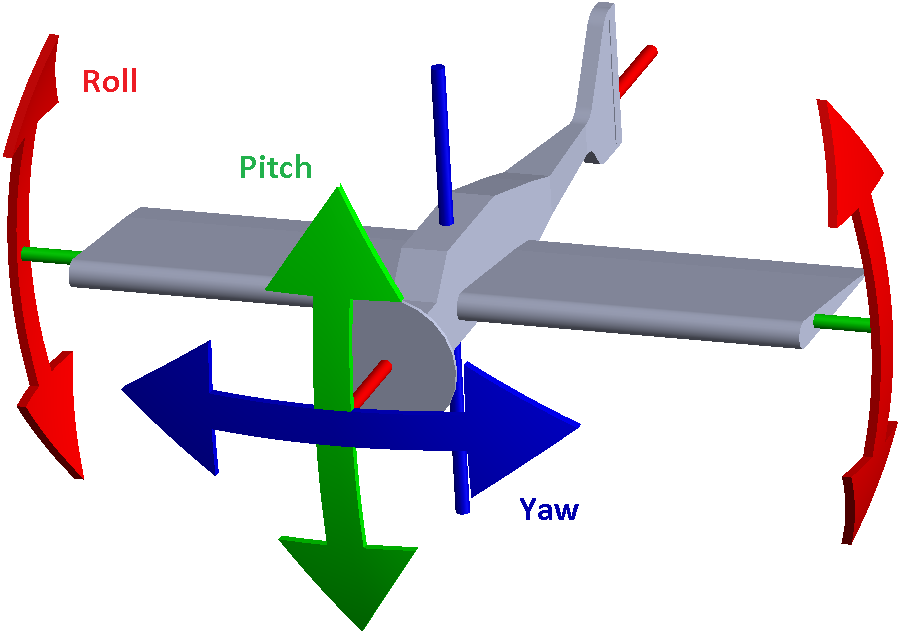
\includegraphics[width=1.0\linewidth]{images/concept/yaw_pitch_roll.png}
	\caption[Steuermanöver]{Mögliche Steuermanöver einer Drohne (Quelle: \fullcite{IaTsI_2015-03-25})}
\end{wrapfigure}
Analog zum Thrust bedeutet eine flache Drehung der Hand (Drehung an der vertikalen Rotations-Achse) eine entsprechende Richtungsänderung der Drohne.

\subsubsection{Pitch (Neigung) / Roll (Rolle)}
Beim Pitch und Roll dreht sich die Drohne um eine horizontale Rotations-Achse. Beim Pitch hebt oder neigt die Drohne ihre Front. Bei Roll sinkt oder erhebt sich eine Seite.

\subsubsection{Finish}
Befindet sich die Drohne im \textit{flugbereiten Zustand (Z2)}, kann via eine Faust-Geste, die Steuerung abgebrochen werden.
Die Drohne reagiert bis zum nächsten \textit{Init-Prozess} nicht mehr.

\newpage
\subsection{Zustands Übersicht}
\label{sec:concept:stateoverview}
%Die Drohne kann aus Sicht der Steuerung, insofern sie eingeschaltet ist, vier Zustände einnehmen:
Die Steuerung kann sich, insofern sie eingeschaltet ist, in vier Zuständen (Z1 -- Z4) befinden:

\begin{figure}[H]
	\centering
	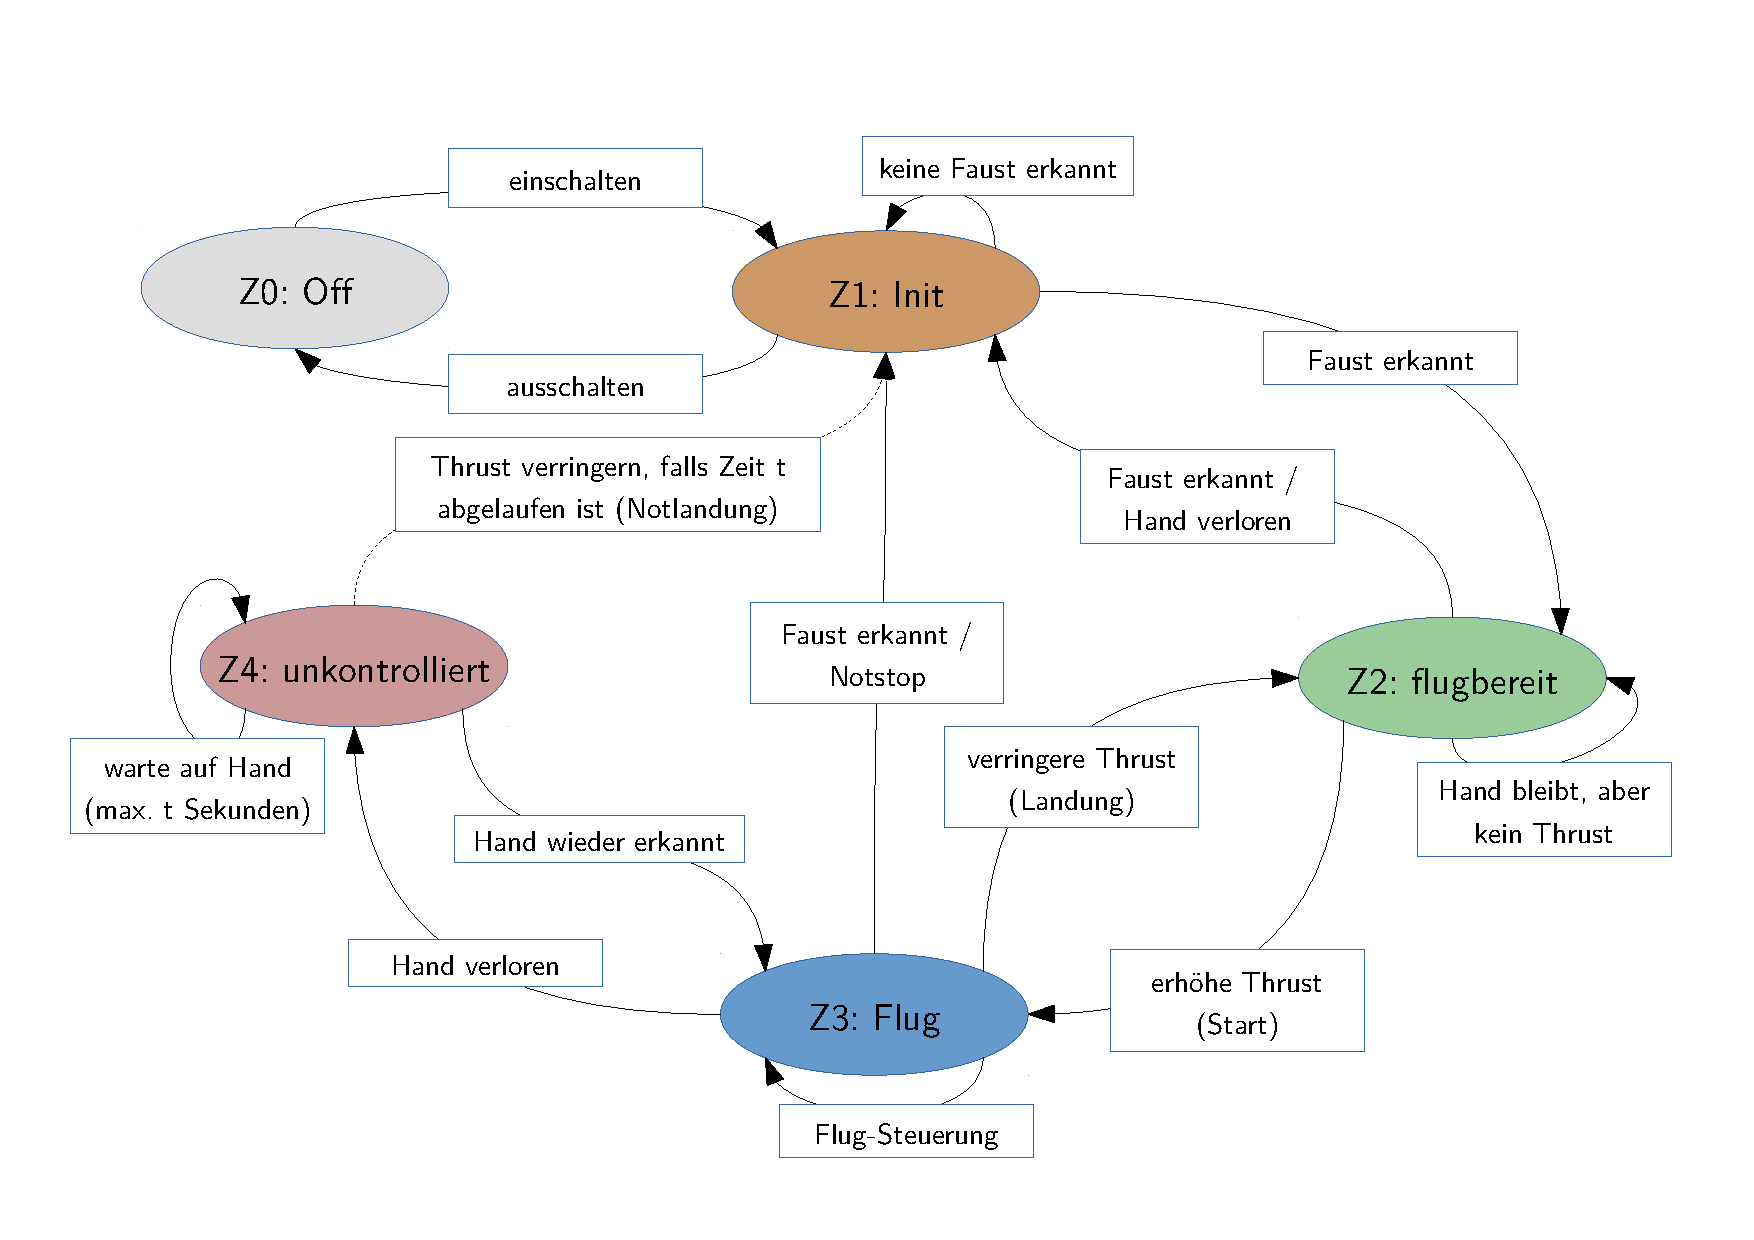
\includegraphics[width=1.0\textwidth]{figures/concept/state-diagram-1.pdf}
	\caption{Zustands-Diagramm: Steuerlogik}
\end{figure}

\subsubsection{Off-Zustand (Z0)}
Die Drohne ist ausgeschaltet.

\subsubsection{Init-Zustand (Z1)}
Die Drohne kann nicht geflogen werden, sondern eine Hand muss zuerst in der initialen Position erkannt werden.

\subsubsection{Flugbereiten Zustand (Z2)}
Die Drohne fliegt nicht, hat aber eine korrekt initialisierte Hand für die Steuerung registriert. Dies kann nach und vor einem Flug sein.

\subsubsection{Flug-Zustand (Z3)}
Die Drohne befindet sich in der Luft.

\subsubsection{Unkontrollierten Zustand (Z4)}
%todo correct
Die Hand wird während dem Flug nicht mehr erkannt oder die Verbindung zur Drohne ist temporär unterbrochen.
Um solche Aussetzer überbrücken zu können, soll sich die Drohne beim Auftreten eines eben genannten Ereignisses, für ca. 2 Sekunden in der Luft halten.
Falls sich das Problem nicht innerhalb einer bestimmten Zeit auflöst, soll die Drohne notgelandet werden, resp. werden die Rotoren ausgeschaltet).

%%%

%todo
\section{Problembehandlung}
Während den verschiedenen Zustände können verschiedene Fehler auftreten:

\subsubsection{Init-Zustand (Z1)}

\begin{table}[H]
	\centering
	\small\renewcommand{\arraystretch}{1.4}
	\rowcolors{1}{tablerowcolor}{tablebodycolor}
	%
	\captionabove{Problem: \textit{Init-Zustand (Z1)} -- Hand-Erkennung}
	%
	\begin{tabularx}{0.9\textwidth}{ L{0.121\linewidth} | X  }%
		\hline
		Problem: & Faust wird nicht erkannt oder mehrere Hände werden erkannt.\\
		Risiko: & \textit{gering}\\
		Folge: & Die Drohne kann nicht abheben. Der \textit{Init-Zustand (Z1)} wird belassen.\\
		\hline
	\end{tabularx}
\end{table}



\subsubsection{Flugbereiten Zustand (Z2)}

\begin{table}[H]
	\centering
	\small\renewcommand{\arraystretch}{1.4}
	\rowcolors{1}{tablerowcolor}{tablebodycolor}
	%
	\captionabove{Problem: \textit{Flugbereiten Zustand (Z2)} -- Hand-Erkennung}
	%
	\begin{tabularx}{0.9\textwidth}{ L{0.121\linewidth} | X  }%
		\hline
		Problem: & Die Hand wird nicht mehr erkannt.\\
		Risiko: & \textit{gering}\\
		Folge: & Die Drone setzt sich zurück in den \textit{Init-Zustand (Z1)}. (Die Drohne befindet sich noch auf dem Boden.)\\
		\hline
	\end{tabularx}
\end{table}


\subsubsection{Flug-Zustand (Z3)}

\begin{table}[H]
	\centering
	\small\renewcommand{\arraystretch}{1.4}
	\rowcolors{1}{tablerowcolor}{tablebodycolor}
	%
	\captionabove{Problem: \textit{Flug-Zustand (Z3)} -- Verbindungsunterbruch}
	%
	\begin{tabularx}{0.9\textwidth}{ L{0.121\linewidth} | X  }%
		\hline
		Problem: & Die Verbindung zwischen Drohne und Steuerung wird unerwartet unterbrochen.\\
		Risiko: & \textit{gering}\\
		Verhalten: &
		Wie im \secref{subsec:isAnalyseDrone} unter API beschrieben, gilt ein Steuerbefehl für 500\,ms.
		Wird die Verbindung unterbrochen, fliegt die Drohne daher maximal eine halbe Sekunde unkontrolliert, bevor die Rotoren ausgeschaltet werden und die Drohne abstürzt. Da die Zustände nur aus der Steuerungssicht existieren, muss die Drohne erneut verbunden und initialisiert werden.\\
		Folge: & Die Drohne wird nach max. 500\,ms unkontrolliert notgelandet.\\
		\hline
	\end{tabularx}
\end{table}


\begin{table}[H]
	\centering
	\small\renewcommand{\arraystretch}{1.4}
	\rowcolors{1}{tablerowcolor}{tablebodycolor}
	%
	\captionabove{Problem: \textit{Flug-Zustand (Z3)} -- Hand-Erkennung}
	%
	\begin{tabularx}{0.9\textwidth}{ L{0.121\linewidth} | X  }%
		\hline
		Problem: & Die Hand wird nicht mehr erkannt oder mehrere Hände werden erkannt.\\
		Risiko: & \textit{sehr gross}\\
		Verhalten: & Der Thrust wird sofort auf mässiges Level getrimmt. Falls länger als $t$ Sekunden keine Hand erkannt wird, werden die Rotoren ausgeschaltet. Die Drohne wechselt in den Init-Zustand (Z1).\\
		Folge: & Die Drohne befindet sich ungesteuert in der Luft oder wird notgelandet (resp. stürzt ab).\\
		\hline
	\end{tabularx}
\end{table}


\begin{table}[H]
	\centering
	\small\renewcommand{\arraystretch}{1.4}
	\rowcolors{1}{tablerowcolor}{tablebodycolor}
	%
	\captionabove{Problem: \textit{Flug-Zustand (Z3)} -- Ruckartige Bewegungen}
	%
	\begin{tabularx}{0.9\textwidth}{ L{0.121\linewidth} | X  }%
		\hline
		Problem: & Starke, unkontrollierte und ruckartige Steuerschwankungen (z.B. aus Angst-Reaktionen etc.).\\
		Risiko: & \textit{erheblich}\\
		Verhalten: & Die Steuerung reguliert, resp. vermeidet sprunghafte Steuerbefehle.\\
		Folge: & Kunstflüge mit bewussten schnellen Anweisungen sind nicht möglich.\\
		\hline
	\end{tabularx}
\end{table}
%

\section{Tests}
% Um die Funktionsweise des ganzen Projekt zu überprüfen, ergeben sich aus logischer Sicht drei einzelne, testbare Komponenten: die Gestenerkennung, der Commander und die Drohne.
Um die Funktionsweise über das ganzen Projekt zu gewährleisten, werden verschiedene Tests im \chapref{chap:testing} durchgeführt.

Für alle Testfälle werden die erwarteten Verhalten, resp. Resultate vorläufig definiert.
Nach der Umsetzung werden alle Tests vollzogen, wobei das erhaltene Resultat mit dem erwarteten Resultat verglichen wird.
Bei Differenzen wird entweder der Fehler behoben und der Test muss erneut durchgeführt werden oder es erfolgt eine genaue Stellungsnahme.

Der Testpool wurde während der Konzeptphase aufgebaut und in der Umsetzungsphase mit weitere sinnvolle Tests ergänzt.
